\ofsection{Game Master}
%
\ofquote{"Tough... Don't blame us. Blame yourself or God."\\}{Delita}\\\\
%
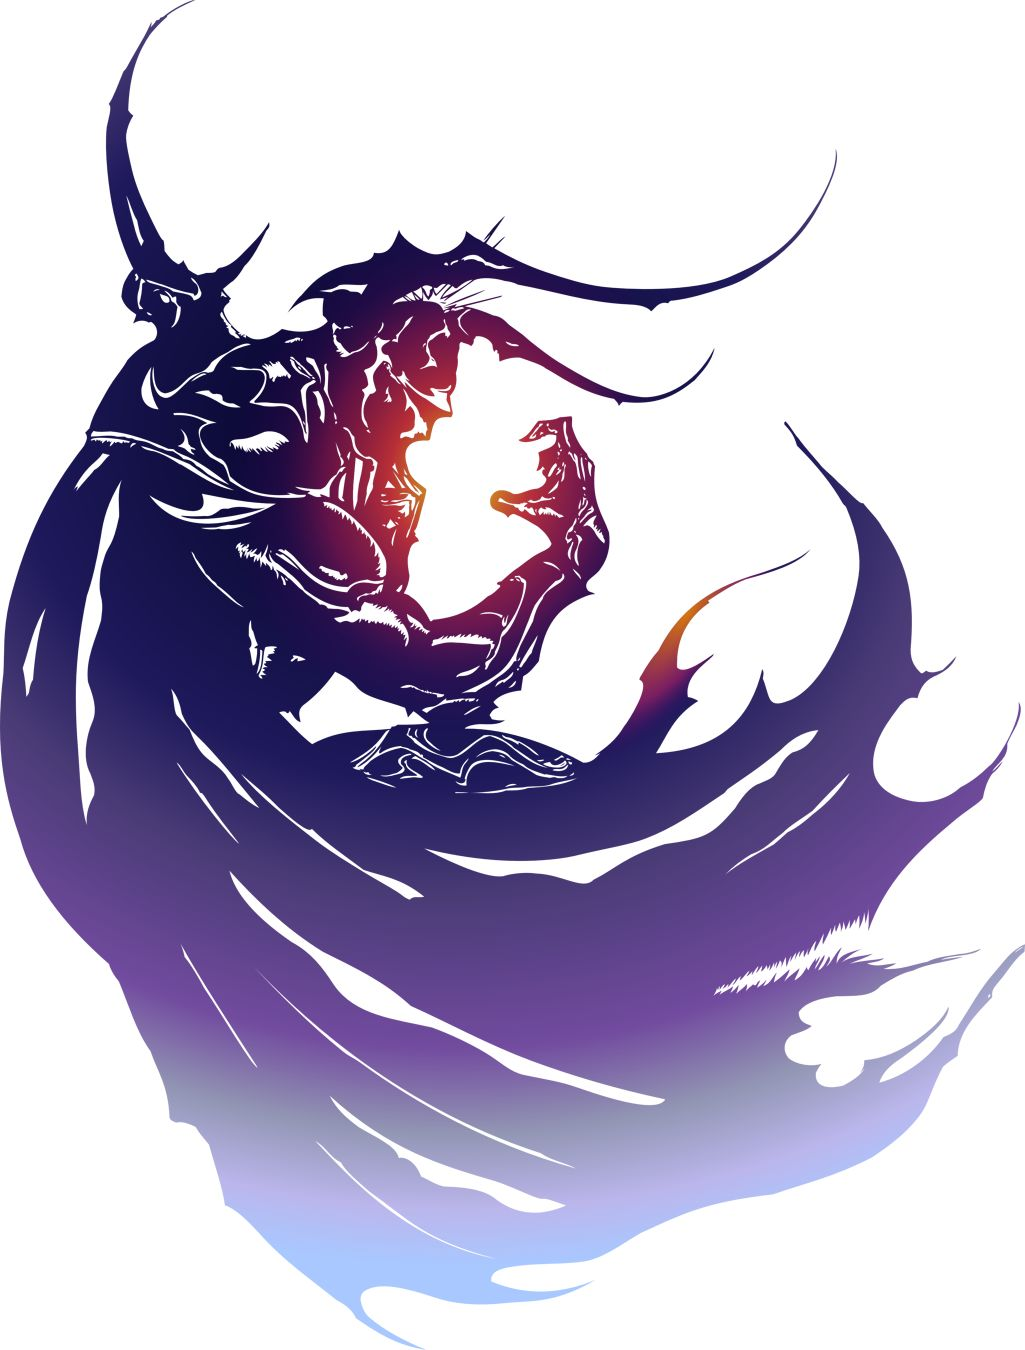
\includegraphics[width=\columnwidth]{./art/images/ff4.jpg}
%
\vfill
%
The \accf{Game Master} creates the setting of the adventure and takes the role of all non-player characters.
Furthermore, the GM describes the environment around the protagonists and decides the outcomes of most actions by applying the rules of the game. 
However, unlike the players, the GM is not strictly bound by rules and may make his own rulings when necessary.
There is no single way to be a successful GM and we encourage you adopt a style that brings enjoyment to both you and the players.
%
\vfill
%
Accordingly, this chapter does not focus on presenting rules or advice.
Instead, it is a collection of optional \accf{supplements}, that you can either use directly or regard as examples for creating your own content.
These supplements not only give a glimpse into the various aspects of game mastering, but also show different directions that you can take as a GM. 
The present modules can be broadly split into two categories: \accf{prepared content} and \accf{optional rules}.
The former provide you with world building blocks such as adventures, settings and monsters that are self-contained and extensible.
The latter present you examples to customize the rules to your preferences by changing or adding to existing ones.
While the prepared content is well suited for beginners, we recommend to consider optional rules once you have gathered some experience.
All available supplements are listed in the following, together with a short synopsis for each one.
%
\newpage
%
{\large\accf{Prepared Content:}}
%
\vfill
%
\accf{Bestiary:} discusses guidelines for creating monsters and combat encounters.
Also includes a collection of prepared enemies that you can use directly.
%
\vfill
%
\accf{Chaos in Cornelia:} a short adventure in which the party has to save a kidnapped princess. 
Contains diverse content including combat, roleplaying and exploration. Highly recommended for beginners!
%
\vfill
%
\accf{Tomb of Raithwall:} a short adventure in which the party has to recover an artifact from a dangerous tomb.
Focused on exploring an environment full of traps and adversaries. 
%
\vfill
%
\accf{Maria \& Draco:} a single-session adventure in which the party has to ensure the success of an opera performance.
Encourages a light-hearted narrative with interesting roleplaying moments.
%
\vfill
%
\accf{Siege of Dollet:} a single-session adventure in which the party has to pass a test to join an elite mercenary force.
Encourages an action packed narrative with lots of combat.
%
\vfill
%
\accf{Gold Saucer:} an amusement park where the party can blow off steam and win rare prizes. 
Focused on recreating the games and competitions in the park.  
%
\vfill
%
\accf{Ivalice Worldbook:} a very detailed document that fleshes out the world of Ivalice, including its history and geography.
You can create various adventures in this world or use it as an example for creating a detailed setting.
%
{\large\ofpar\ofrow\accf{Optional Rules:}}
%
\vfill
%
\accf{Additional Rules:} minor rule changes and additions that help you to customize the feeling of the game.
%
\vfill
%
\accf{Races:} rules and examples for incorporating different humanoid races in your world. 
This provides additional character creation options for players, but can also help you to create a more interesting game world.
%
\vfill
%
\accf{Chocobo:} rules for incorporating bird-like creatures called Chocobos as full-fledged party members.
Players can raise Chocobos, use them as mounts and fight alongside them in combat.
%
\vfill
%
\accf{Triple Triad:} rules for a fun card game, allowing the party to collect and play cards.
Well suited if you are looking quick and simple side-activity for the party.
%
\vfill
%
\accf{Blitzball:} rules for a fun team-based sports game similar to water polo.
Well suited if you are looking for a more elaborate side-activity for the party.
%
\clearpage